% LaTeX source for ``การเรียนรู้ของเครื่องสำหรับเคมีควอนตัม (Machine Learning for Quantum Chemistry)''
% Copyright (c) 2022 รังสิมันต์ เกษแก้ว (Rangsiman Ketkaew).

% License: Creative Commons Attribution-NonCommercial-NoDerivatives 4.0 International (CC BY-NC-ND 4.0)
% https://creativecommons.org/licenses/by-nc-nd/4.0/

\chapter{การเรียนรู้ของเครื่อง}
\label{ch:ml}

\idxboth{การเรียนรู้ของเครื่อง}{Machine Learning}
\idxboth{การฝึกสอนโมเดล}{Model Training}

%--------------------------
\section{ความสำคัญของการเรียนรู้ของเครื่อง}
%--------------------------

\begin{figure}[H]
    \centering
    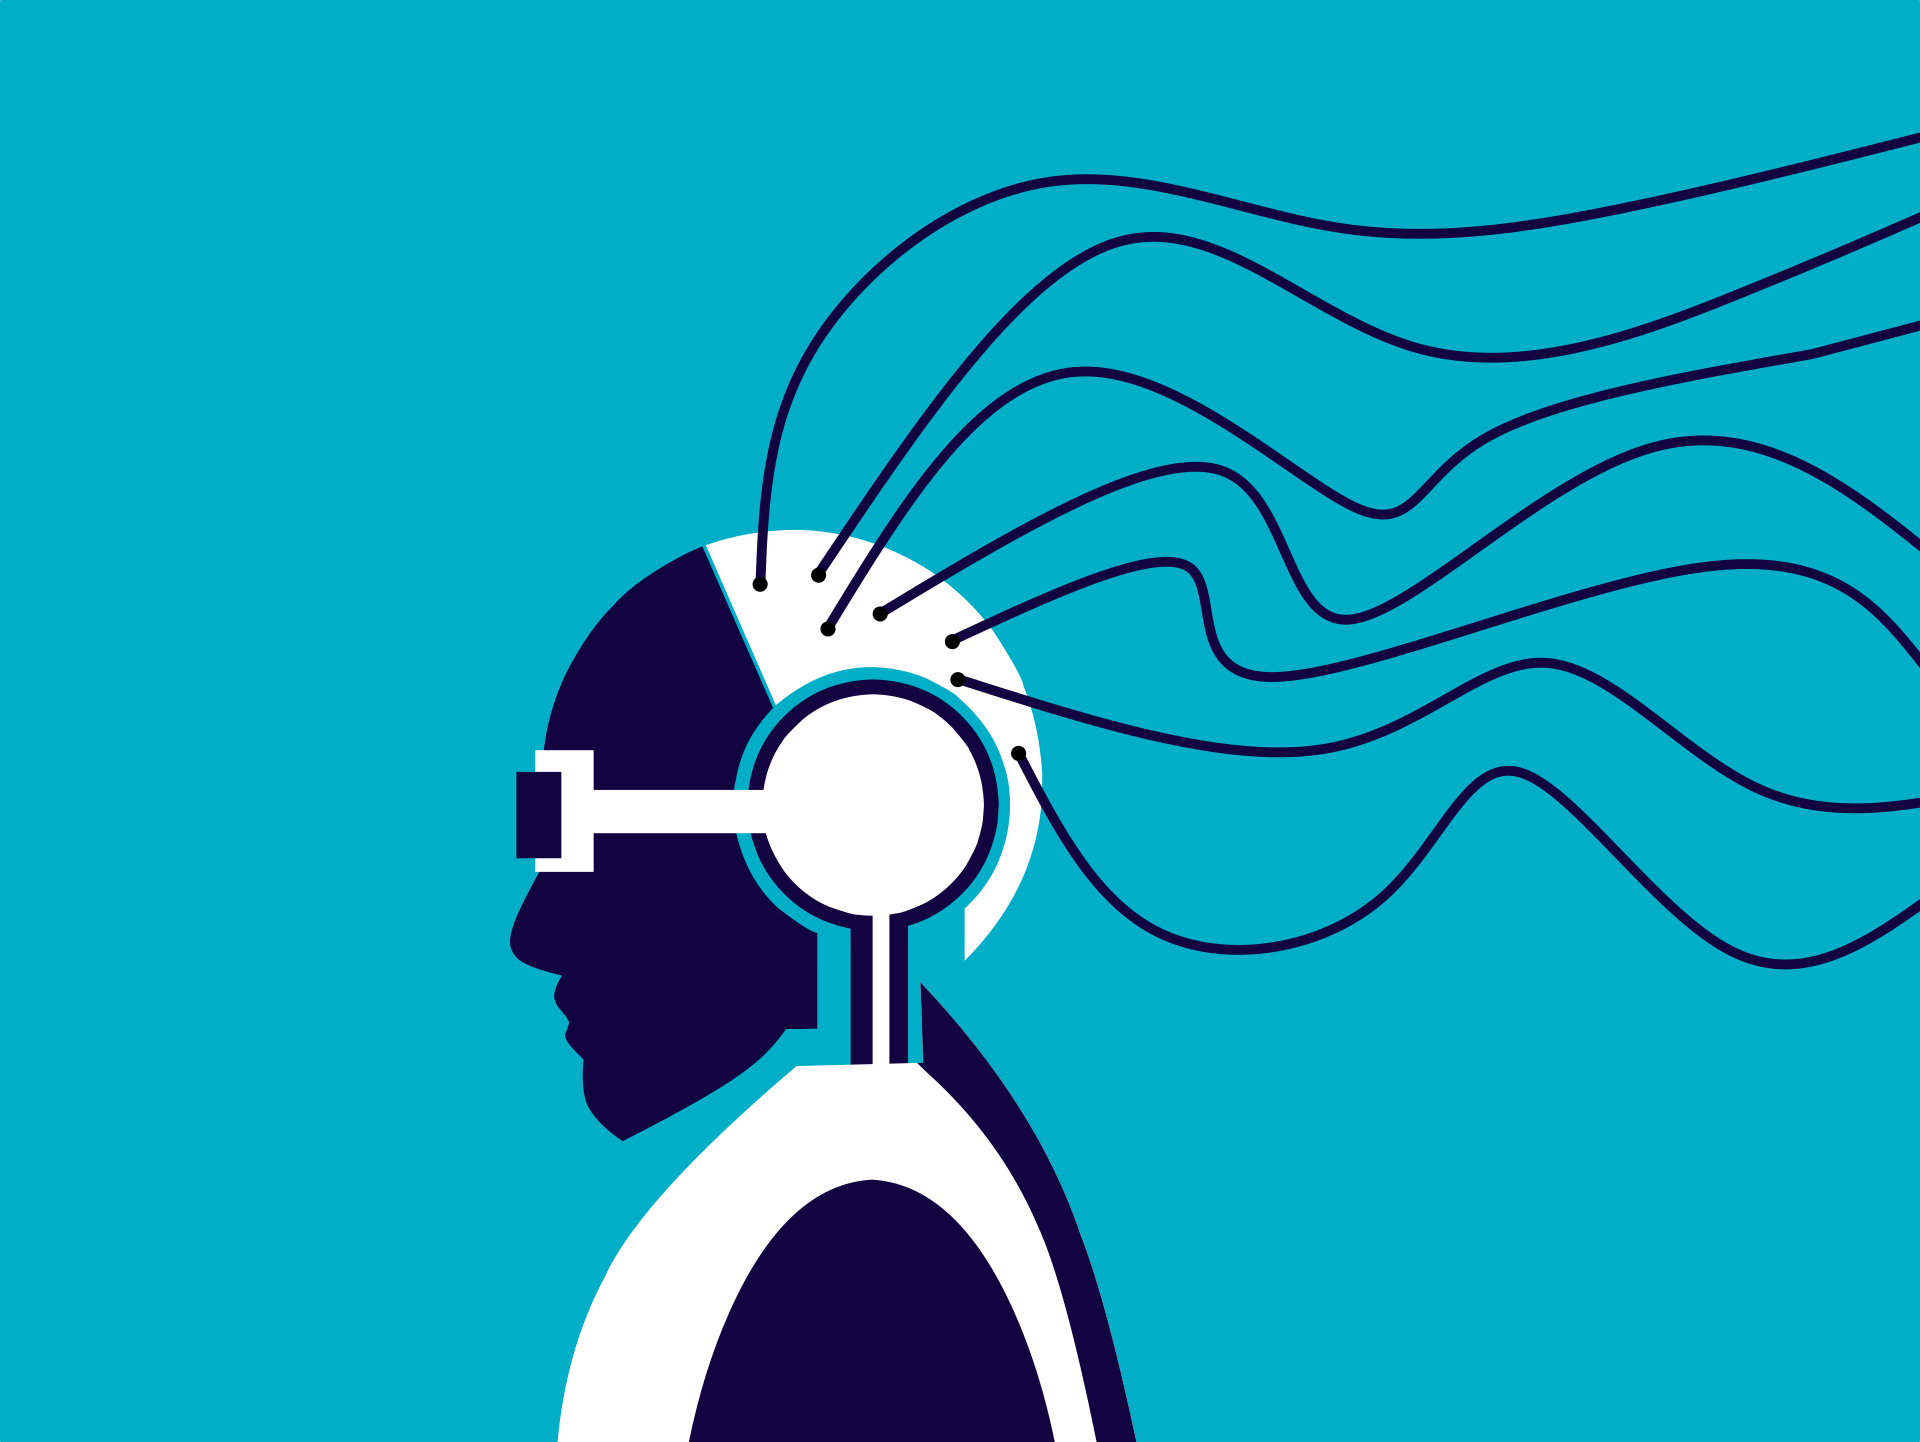
\includegraphics[width=0.8\linewidth]{fig/cyborg.png}
    \caption{ภาพแสดงหุ่นยนต์ที่มีสมองที่มีความนึกคิดและสติปัญญา (เครดิตภาพ: https://pixabay.com)}
    \label{fig:cyborg}
\end{figure}

การเรียนรู้ของเครื่องหรือ Machine Learning (ML) เป็นศาสตร์ที่เชื่อมโยงวิชาสถิติ คณิตศาสตร์ และวิทยาการคอมพิวเตอร์เข้าด้วยกัน
กล่าวคือมนุษย์พยายามทำให้เครื่องจักรนั้นมี \enquote{สติปัญญา} หรือ \enquote{ความฉลาด} เหมือนมนุษย์ และมีความสามารถในการเรียนรู้สิ่งต่าง ๆ 
ได้ด้วยตัวเอง โดยกระบวนการดังกล่าวนั้นจะเกี่ยวข้องกับการฝึกสอนเครื่องจักรจนกระทั่งเครื่องจักรสามารถเรียนรู้และค่อย ๆ พัฒนาการทำงานต่าง ๆ 
ได้โดยไม่ต้องพึ่งการตั้งโปรแกรม ซึ่งในบริบทนี้เครื่องจักรที่เรารู้จักกันดีก็คืออุปกรณ์ที่มีหน่วยประมวล (Processing Unit) เช่น คอมพิวเตอร์ 
ที่ถูกสั่งงานหรือควบคุมผ่านซอฟต์แวร์ในรูปแบบของโปรแกรมนั่นเอง โดยวิธีการก็คือเราป้อนข้อมูลเข้าไปให้กับโปรแกรม โปรแกรมจะทำการสร้างโมเดล
(Model) ที่สามารถอธิบายความสัมพันธ์ในข้อมูลที่เราป้อนเข้าไปได้ ซึ่งขั้นตอนที่เกิดขึ้นระหว่างการเรียนรู้ก็คือการฝึกสอนโมเดล (Model Training) 
ซึ่งโปรแกรมสามารถแปลงข้อมูลทั้งหมดเป็นโมเดลที่ปรับปรุงได้ นั่นหมายความว่าเทคโนโลยีการเรียนรู้ของเครื่องสามารถทำให้คอมพิวเตอร์เรียนรู้วิธีทำงาน%
ของมนุษย์โดยเฉพาะกิจกรรมที่ทำซ้ำหรือเกิดขึ้นแบบเดิมจนมีแบบแผน (Pattern) ที่สามารถเลียนแบบได้นั่นเอง อธิบายง่าย ๆ ก็คือถ้าเรามีข้อมูล 2 
ตัวแปร $(x,y)$ เราใช้ ML เพื่อหาฟังก์ชันที่สามารถเชื่อมโยง (Correlate) ความสัมพันธ์ระหว่างสองตัวแปรนี้ได้ $f: x\rightarrow y$

ML ได้ถูกพัฒนาเรื่อยมาเป็นระยะเวลาหลายทศวรรษ จุดเริ่มต้นที่นับได้ว่าสำคัญที่สุดของปัญญาประดิษฐ์เกิดขึ้นในปี ค.ศ. 1943 โดยนักตรรกศาสตร์
Walter Pitts และนักประสาทวิทยา Warren McCulloch ได้ตีพิมพ์ผลงานที่เสนออัลกอริทึมคณิตศาสตร์ของโครงข่ายประสาท (Neural Network) 
และในปี ค.ศ. นักคณิตศาสตร์และนักถอดรหัสชื่อดัง Alan Turing\footnote{Alan Turing เป็นอัจฉริยะด้านคณิตศาสตร์และคำนวณ จบการศึกษา%
ปริญญาตรีจาก University of Cambridge และปริญญาเอกจาก Princeton University โดยในช่วงสงครามโลก Alan ได้สร้างเครื่องถอดรหัส%
ที่ชื่อว่า Bombe เพื่อมาต่อสู้กับเครื่อง Enigma ซึ่งได้การประเมินไว้ว่าผลงานของ Alan ได้ช่วยชีวิตไว้ได้หลายล้านคน} ได้เสนอ The Turing Test 
ซึ่งเป็นแนวคิดที่สามารถนำมาใช้ในการทดสอบความมีสติปัญญาของเครื่องจักร หลังจากนั้นได้มีเหตุการณ์สำคัญเกิดขึ้นอีกมากมาย เช่น Arthur Samuel 
ได้เขียนโปรแกรมเล่นหมากฮอสโปรแกรมโปรแกรมแรกของโลกให้กับ IBM ในปี ค.ศ. 1952 และ อัลกอริทึม Nearst Neighbor ถูกคิดค้นขึ้นในช่วงปี 
ค.ศ. 1967 และในปี ค.ศ. 1996 บริษัท IBM ได้พัฒนาโปรแกรมที่ชื่อว่า Deep Blue ที่สามารถเอาชนะนักหมากรุกมือวางอันดับหนึ่งของโลกได้สำเร็จ

\begin{figure}[H]
    \centering
    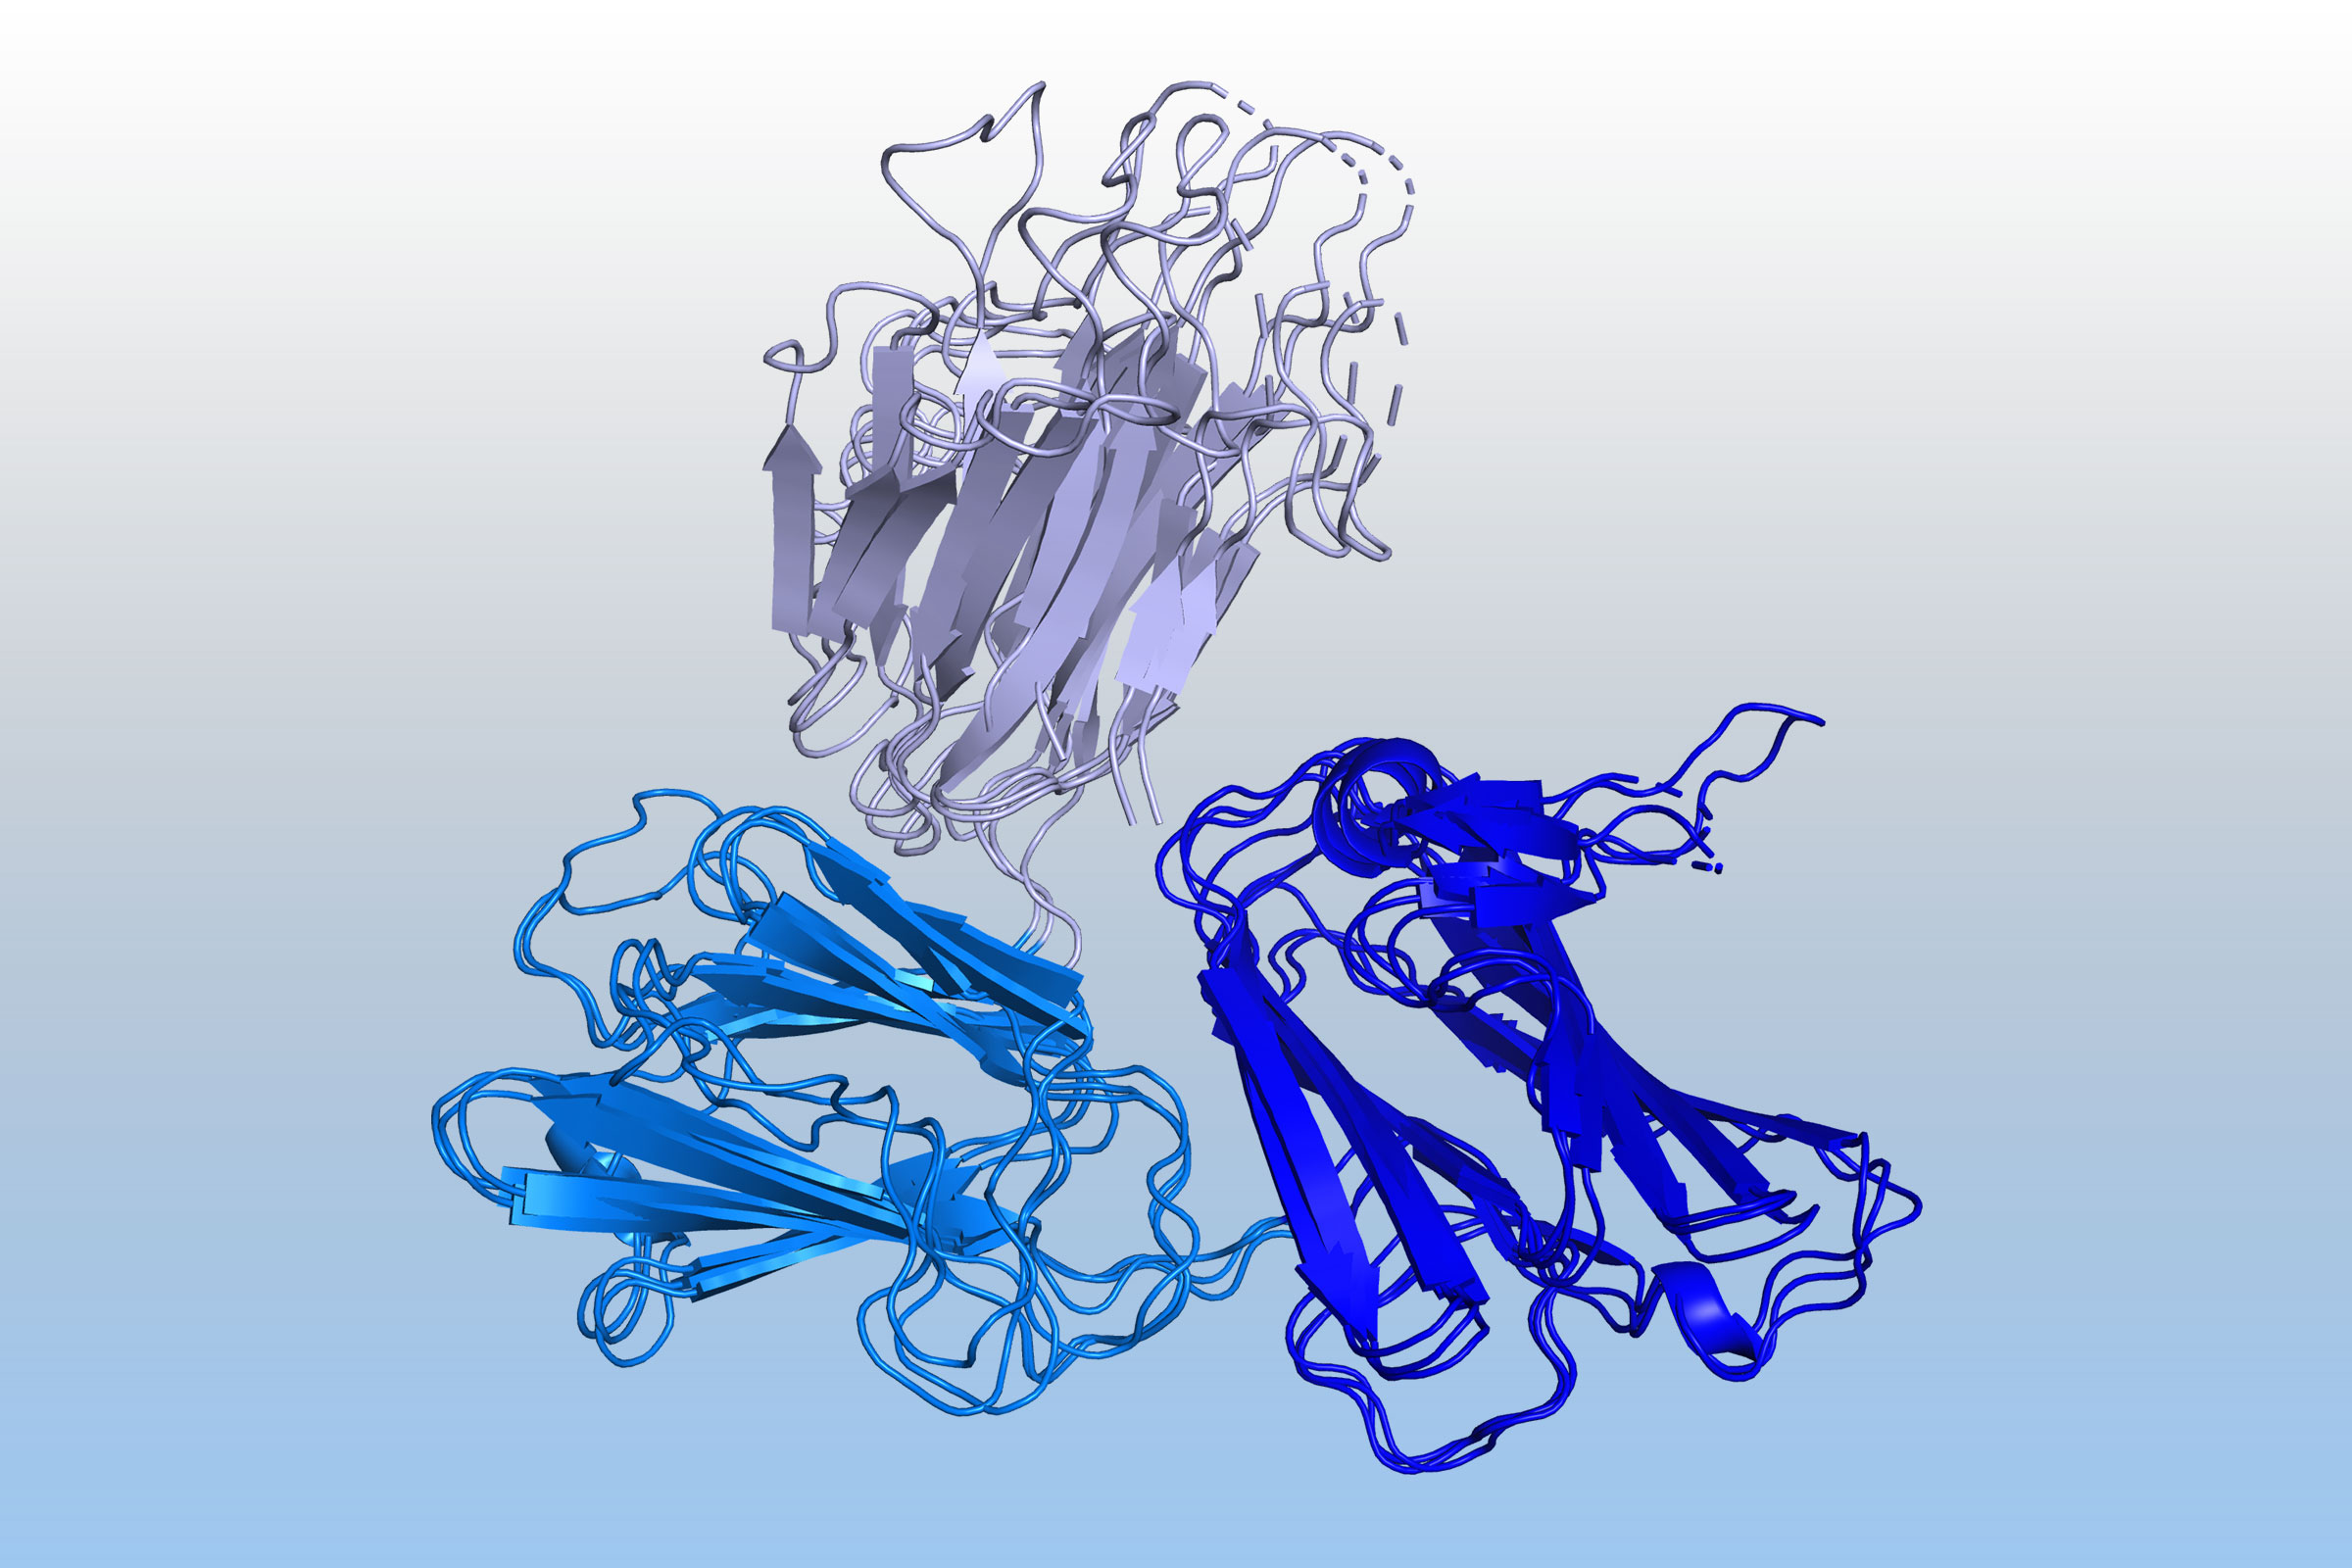
\includegraphics[width=\linewidth]{fig/malaria-parasite-protein-deepmind.jpeg}
    \caption{แบบจำลองโครงสร้างสามมิติการพับของโปรตีน Pfs48/45 ซึ่งเป็นองค์ประกอบสำคัญของปรสิตมาลาเรีย โครงสร้างนี้ทำนายด้วยโมเดล 
    ปัญญาประดิษฐ์ AlphaFold ซึ่งถูกพัฒนาโดย DeepMind (เครดิตภาพ: DeepMind)}
    \label{fig:malaria_parasite}
\end{figure}

นับตั้งแต่ปี ค.ศ. 2000 เป็นต้นมานั้นเรียกได้ว่าเป็นช่วงของการพัฒนาปัญญาประดิษฐ์แบบสมัยใหม่ก็ว่าได้ จุดเปลี่ยนที่น่าสนใจที่ทำให้คนหันมาสนใจ%
และให้ความสำคัญกับ ML ก็คือในช่วงระยะเวลา 10 ปีที่ผ่านมาได้มีเหตุการณ์สำคัญที่สร้างแรงกระเพื่อมแก่มวลมนุษยชาติ เช่น ในปี ค.ศ. 2011 
Apple ได้ปล่อยผลิตภัณฑ์ที่ชื่อ Siri ซึ่งเป็นผู้ช่วยเสมือน (Intelligent Virtual Assistant) อันแสนฉลาดออกมา และในปี ค.ศ. 2016 
บริษัท DeepMind ซึ่งเป็นบริษัทลูกของ Alphabet ก็พัฒนาโมเดลปัญญาประดิษฐ์ AlphaGo ที่สามารถเล่นหมากล้อมได้อย่างชาญฉลาด 
และก็เป็นปีเดียวกันกับที่ DeepMind ได้เริ่มต้นพัฒนา AlphaFold ซึ่งเป็นโมเดล ML สำหรับการทำนายโครงสร้างสามมิติของโปรตีน และในปี ค.ศ. 
2021 DeepMind ก็ได้ตีพิมพ์บทความที่นำเสนอ AlphaFold 2 ออกมาครับ\autocite{jumper2021} 
\footnote{
\setlength\intextsep{0pt}
\begin{wrapfigure}{r}{0.2\textwidth}
        \centering
        
\includegraphics[width=0.18\textwidth]{fig/qr_code_alphafold2_explained.png}
\end{wrapfigure}
ถ้าหากใครที่อ่านบทความแล้วยังไม่เข้าใจก็สามารถดูวิดีโอบน YouTube \enquote{DeepMind's AlphaFold 2 Explained! 
AI Breakthrough in Protein Folding! What we know (\& what we don't)} ที่อธิบายโดย Yannic Kilcher ได้โดยสแกน 
QR Code ทางด้านขวา}

ช่วงปลายปี ค.ศ. 2022 ทีม DeepMind ก็ได้สะเทือนวงการปัญญาประดิษฐ์อีกครั้งด้วยอัลกอริทึมการเรียนรู้ของเครื่องแบบใหม่ที่สามารถหาอัลกอริทึม%
ที่สามารถคูณเมทริกซ์ได้โดยมีความเร็วมากกว่าอัลกอริทึมแบบดั้งเดิมที่ใช้กันมายาวนานกว่า 50 ปี โดยโมเดลที่ทาง DeepMind ได้สร้างขึ้นมานั้นมีชื่อว่า
AlphaTensor โดยใช้ Transformer\autocite{vaswani2017} เป็นโมเดลหลักในการฝึกสอน\footnote{โมเดลการเรียนรู้เชิงลึกแบบหนึ่งซึ่งใช้ 
Self-attention พัฒนาโดย Google Brain สำหรับงานทางด้าน Natural Language Processing หรือ NLP และเผยแพร่ในปี ค.ศ. 2017}
โดยอัลกอริทึมที่ถูกค้นพบโดย AlphaTensor นั้นสามารถทำการคูณเมทริกซ์ขนาด $4 \time 4$ ได้โดยใช้การคูณทั้งหมดแค่ 47 ครั้ง 
ซึ่งน้อยกว่าการใช้อัลกอริทึมของสตราซเซนแบบสองระดับ (Strassen's Two-level Algorithm)\autocite{strassen1969} 
ซึ่งใช้การคูณทั้งหมด 49 ครั้ง และค่าความซับซ้อนเชิงการคำนวณ (Computational Complexity) ของอัลกอริทึมใหม่นี้อยู่ที่ประมาณ 
${\mathcal{O}}({N}^{2.778})$ 

จากตัวอย่างข้างต้นนั้นเราสามารถสรุปได้อย่างไม่ต้องลังเลเลยว่าการเรียนรู้ของเครื่องนั้นสามารถปฏิวัติวงการต่าง ๆ ได้อย่างน่าเหลือเชื่อ
ไม่เพียงเฉพาะวงการคณิตศาสตร์และวิทยาศาสตร์เท่านั้น แต่รวมไปถึงวงการอื่น ๆ ด้วยที่เทคนิคเหล่านี้เข้าไปมีบทบาท ซึ่งไม่เพียงแค่ในเฉพาะปัจจุบันเท่านั้น
แต่ว่าในอนาคตนั้นเราอาจจะได้เห็นสิ่งใหม่ ๆ ที่ปัญญาประดิษฐ์นั้นสามารถสร้างสรรค์ขึ้นมา

\begin{figure}[H]
    \centering
    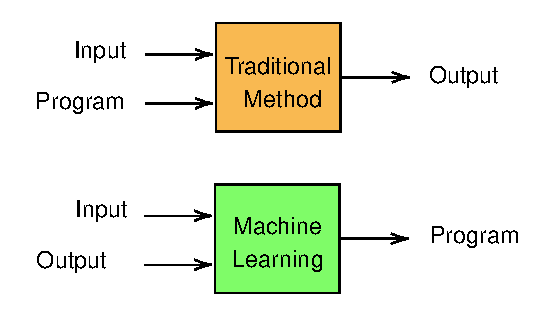
\includegraphics[scale=1]{fig/ML-concept.pdf}
    \caption{แผนภาพเปรียบเทียบการทำงานของโปรแกรมแบบดั้งเดิมกับการเรียนรู้ของเครื่อง}
    \label{fig:ml_paradigm}
\end{figure}

แผนภาพที่ \ref{fig:ml_paradigm} แสดงโมเดลเปรียบเทียบอินพุตและเอาต์พุตของโปรแกรมคอมพิวเตอร์ทั่วไปและปัญญาประดิษฐ์ โดยการเขียน%
โปรแกรมแบบทั่วไปหรือดั้งเดิมนั้นเราจะต้องทำการเขียนโปรแกรมเริ่มต้นขึ้นมาและทำการป้อนอินพุตเข้าไปเพื่อให้ได้มาซึ่งคำตอบที่เราต้องการ โดยกระบวน%
ของการเขียนโปรแกรมแบบดั้งเดิมนี้จะเป็นแบบทำแล้วจบ พูดง่าย ๆ คือโปรแกรมของเราถูกกำหนดมาให้เพื่อให้รับอินพุตและคำนวณเอาต์พุตแบบเดียว
ซึ่งเราไม่สามารถนำโปรแกรมที่เขียนขึ้นมานี้ไปใช้ต่อได้ (Non-transferable) แต่สำหรับปัญญาประดิษฐ์นั้นจะตรงข้ามกัน เราจะมีการป้อนทั้งอินพุต%
และเอาต์พุตเข้าไปและให้ปัญญาประดิษฐ์ทำการสร้างโปรแกรมหรือโมเดลที่สามารถอธิบายความสัมพันธ์ของชุดข้อมูลที่มีตัวแปรต้นและตัวแปรตามได้ 
ซึ่งโมเดลที่ถูกสร้างขึ้นมาสามารถนำไปใช้งานต่อได้กับชุดข้อมูลอื่น (Transferable)

%--------------------------
\section{เมื่อการเรียนรู้ของเครื่องมาเจอกับเคมี}
%--------------------------

\begin{figure}[H]
    \centering
    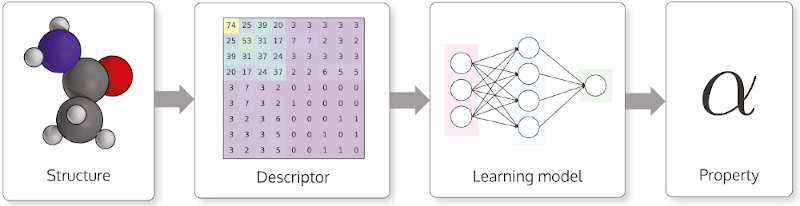
\includegraphics[width=\linewidth]{fig/workflow_chem_ml.png}
    \caption{ขั้นตอนแสดงการสร้างโมเดลการเรียนรู้ของเครื่องเพื่อใช้ในการทำนายคุณสมบัติของโมเลกุล เริ่มจากการเปลี่ยนข้อมูลทางเคมีจาก%
    จากโครงสร้างของโมเลกุลไปเป็นข้อมูลแบบดิจิตอลที่คอมพิวเตอร์สามารถเข้าใจและประมวลผลต่อได้ ตามด้วยขั้นตอนการสร้างโมเดลสำหรับ%
    การเรียนรู้ และขั้นตอนสุดท้ายคือการทำนายคุณสมบัติของโมเลกุล (เครดิตภาพ: https://chemintelligence.com)}
    \label{fig:workflow_chem_ml}
\end{figure}

เคมีเป็นศาสตร์ที่เสมือนกับเป็นสะพานเชื่อมโยงศาสตร์อื่น ๆ เข้าด้วย พูดง่าย ๆ คือเคมีเป็นสาขาที่อยู่ตรงกลางระหว่างสาขาฟิสิกส์ ชีววิทยา และคณิตศาสตร์
นั่นก็เพราะว่าวิชาเคมีนั้นเป็นการบูรณาการทั้งสามสาขาเข้าด้วยกัน เราใช้ความรู้ทางทฤษฎีโดยเฉพาะกลศาสตร์ฟิสิกส์มาทำความเข้าใจอนุภาคขนาดเล็ก 
อะตอม โมเลกุลอินทรีย์และอนินทรีย์ สารประกอบที่มีความซับซ้อน พอลิเมอร์ที่มีขนาดใหญ่ องค์ประกอบและหน่วยวัสดุต่าง ๆ รวมไปถึงชีวโมเลกุล เช่น 
โปรตีน ลิพิด สารพันธุกรรม ซึ่งเป็นองค์ประกอบขั้นพื้นฐานของสิ่งมีชีวิต และเรายังต้องใช้ความรู้ทางคณิตศาสตร์ในการแก้ปัญหาทางฟิสิกส์เชิงเคมีอีกด้วย

สำหรับปัญญาประดิษฐ์ซึ่งมีการเรียนรู้ของเครื่องเป็นหัวใจสำคัญนั้น ก็ถือว่าเป็นสาขาหนึ่งของวิชาสถิติเชิงข้อมูลและเกี่ยวข้องกับวิทยาการคอมพิวเตอร์
โดยการนำการเรียนรู้ของเครื่องเข้ามาใช้ในการแก้ปัญหาบางอย่างทางเคมีนั้นถือว่าเหมาะสมยิ่ง นั่นก็เพราะว่านักเคมีมีข้อมูลทีได้จากการทดลองอย่างมหาศาล
มีทั้งข้อมูลผลการทดลองที่เป็นบวกก็ดี หรือผลที่เป็นลบก็ดี ซึ่งข้อมูลเหล่านี้นั้นอาจจะข้อมูลเชิงลึกแอบแฝงอยู่ ดังนั้นการเรียนรู้ของเครื่องจึงเข้ามามีบทบาท%
อย่างมากในการสกัดหรือดึงสิ่งที่ซ่อนอยู่ออกมา ทำให้เราเข้าใจข้อมูลทางเคมีมากขึ้นและนำไปสู่การค้นพบหรือการทำนายสิ่งใหม่ ๆ ที่จะช่วยต่อยอดให้%
การทำงานวิจัยทางด้านเคมีนั้นเป็นไปอย่างรวดเร็วอย่างที่เรียกว่าก้าวกระโดดเลยทีเดียว\autocite{cartwright2020,zotero-817}

%--------------------------
\section{บทบาทของการเรียนรู้ของเครื่องต่อเคมีควอนตัม}
%--------------------------

เคมีควอนตัม (Quantum Chemistry) เป็นแขนงหนึ่งของวิชาเคมีเชิงฟิสิกส์ (Physical Chemistry) ซึ่งเป็นการผสมผสานระหว่างกลศาสตร์ควอนตัม 
(Quantum Mechanics) และการศึกษาอะตอมและโมเลกุลเข้าด้วยกัน ซึ่งจะเรียกอีกอย่างว่ากลศาสตร์ควอนตัมโมเลกุลก็ได้เช่นกัน (Molecular 
Quantum Mechanics) อธิบายได้ง่าย ๆ คือเป็นการนำความรู้ทางด้านกลศาสตร์ควอนตัมที่เป็นการศึกษาอันตรกิริยาระหว่างอนุภาคพื้นฐานในอะตอม 
(อิเล็กตรอน โปรตอน และนิวตรอน) มาศึกษาคุณสมบัติโดยรวมของอะตอม โมเลกุล สารประกอบอินทรีย์และอนินทรีย์ สารชีวโมเลกุล หรือวัสดุที่เราสนใจ 
ซึ่งนักวิทยาศาสตร์ได้ศึกษาและค้นคว้างานวิจัยศาสตร์ด้านนี้มากว่าหนึ่งศควรรษ นับตั้งแต่ช่วงต้นปี ค.ศ. 1920 โดยได้มีการพัฒนาทฤษฎีต่าง ๆ มากมาย 
แต่สิ่งที่น่าสนใจก็คือจุดเปลี่ยนที่สำคัญของเคมีควอนตัมยุคใหม่ก็คือ \enquote{ทฤษฎีฟังก์ชันนอลความหนาแน่น} หรือ \enquote{Density Functional 
Theory (DFT)}\autocite{kohn1996} ซึ่งถูกคิดค้นมากว่าครึ่งศตวรรษ และถูกนำมาใช้อย่างแพร่หลายในงานวิจัยทั้งทางด้านเคมีและฟิสิกส์ 
ถ้าหากใครที่เคยเรียนวิชาเคมีเชิงฟิสิกส์หรือฟังการนำเสนอผลงานวิชาการตามงานประชุมวิชาการเคมีก็น่าจะเคยได้ยินชื่อทฤษฎีนี้กันมาบ้าง 
\idxboth{เคมีควอนตัม}{Quantum Chemistry}
\idxboth{ทฤษฎีฟังก์ชันนอลความหนาแน่น}{Density Functional Theory}

DFT เป็นทฤษฎีที่เรานำมาใช้ในการศึกษาคุณสมบัติของโมเลกุล ไม่ว่าจะเป็นขนาดเล็กอย่างเช่นโมเลกุลของสารประกอบอินทรีย์ และอนินทรีย์ 
หรือจะเป็นโมเลกุลขนาดใหญ่ เช่น โปรตีน, วัสดุโลหะ, และพอลิเมอร์ นั่นก็เพราะว่า DFT เป็นวิธีการคำนวณที่ให้ผลแม่นยำและใช้เวลาในการคำนวณ%
ที่ไม่นานมาก นั่นจึงทำให้ทฤษฎี DFT ได้รับการเชิดชูเกียรติด้วยรางวัลโนเบลสาขาเคมีในปี ค.ศ. 1998 โดยผู้รับรางวัลได้แก่ ศาสตราจารย์ Walter 
Kohn (University of California, Santa Barbara, CA, USA) สำหรับการพัฒนาทฤษฎี DFT และศาสตราจารย์ John Pople 
(Northwestern University, Evanston, IL, USA) สำหรับการพัฒนาวิธีการคำนวณในเคมีควอนตัม\footnote{รายละเอียดของรางวัลดูได้ที่ 
\url{https://www.nobelprize.org/prizes/chemistry/1998/summary/}} และถูกนำมาใช้อย่างแพร่หลายในงานวิจัยทางด้านเคมี ฟิสิกส์ 
ชีววิทยา และรวมไปถึงวัสดุศาสตร์ด้วย แต่ทว่าในความเป็นจริงนั้นทฤษฎี DFT ไม่ได้ให้ผลการคำนวณที่แม่นยำสูงมากนักเมื่อเทียบกับวิธีฟังก์ชันคลื่นหรือ 
Wavefunction Theory (WFT) และยังไม่สามารถคำนวณคุณสมบัติของระบบบางระบบได้ จึงทำให้ในปัจจุบันนั้นได้มีการพัฒนาระเบียบวิธีใหม่ ๆ 
ขึ้นมาเพื่อปรับปรุงประสิทธิภาพหรือความสามารถของ DFT ให้เทียบเท่ากับวิธีที่อ้างอิงด้วยวิธี

ในขณะเดียวกันนั้น ML ก็ถูกนำมาใช้ประโยชน์ในงานวิจัยเคมีมานานกว่า 30 ปีแล้ว แต่ในปัจจุบันนั้น เทคโนโลยีต่าง ๆ เช่น Supercomputing Cloud และ 
Graphical Processing Unit (GPU) ได้เข้ามามีบทบาทอย่างมากในวิทยาศาสตร์เชิงคำนวณ (Computaitonal Science) โดยเฉพาะเคมีเชิงคำนวณ 
(Computational Chemistry) จึงทำให้มีจุดเปลี่ยนที่ทำให้ความสนใจของนักวิจัยในช่วง 10 ปีที่ผ่านมานี้ในหันมาทำงานวิจัยโดยใช้ ML กันมากขึ้น 
นั่นก็เพราะว่าในปัจจุบันนั้น ML สามารถศึกษาได้ง่ายขึ้นเมื่อเทียบกับในอดีต ทุกวันนี้เราไม่จำเป็นต้องมานั่งเขียนโค้ดเพื่อสร้างโมเดล ML แบบเริ่มจากศูนย์กันแล้ว 
ตอนนี้เรามี Library แบบ Open-source ต่าง ๆ มากมายให้เลือกใช้ เช่น Scikit-learn\autocite{scikit-learn}, 
TensorFlow\autocite{tensorflow2015-whitepaper}, PyTorch\autocite{NEURIPS2019_9015}, Flux\autocite{innes2018}, 
หรือแม้แต่ Matlab\autocite{MATLAB:2010} ที่ก็มีฟังก์ชันสำเร็จรูปมาให้เราใช้งานได้เลย ซึ่งทำให้เราสามารถเลือกใช้โมเดล ML ต่าง ๆ ได้ตามต้องการ

ผู้เขียนขอยกตัวอย่างงานวิจัยหนึ่งที่ตอนนี้กำลังเป็นหัวข้อที่มาแรง (อย่างน้อย ๆ ก็ ณ วันที่ผู้เขียนกำลังเขียนหนังสือเล่มนี้) นั่นคือการพัฒนาโมเดล ML 
ของฟังก์ชันการแลกเปลี่ยนและสหสัมพันธ์ (Exchange-Correlation Functional หรือ XC) ซึ่งเป็นอินพุตที่สำคัญที่สุดของ DFT เพื่อนำไปศึกษา%
ให้ได้หลายระบบ เช่น โมเลกุล โครงสร้าง และสารประกอบที่มีขนาดเล็กและใหญ่ ซึ่งเราเรียกสิ่งที่มีความสามารถในการทำอะไรได้หลาย ๆ อย่างว่า% 
สารพัดประโยชน์ (General-Purpose) หรือสิ่งที่มีความสากล (Universality) นั่นเอง ซึ่งถ้าหากเราพัฒนาโมเดล XC ด้วย ML ได้สำเร็จหรือมี%
ประสิทธิภาพที่ดีมาก ๆ เราก็จะมีโมเดล XC ที่สามารถนำไปใช้ในการศึกษาคุณสมบัติของโมเลกุลและสารประกอบได้ถูกต้องและแม่นยำ แต่ในความเป็นจริงนั้น 
XC ก็เปรียบเสมือนเป็นกล่องดำ (Black Box) เพราะว่าไม่มีใครที่รู้หน้าตาสมการหรือผลเฉลยทั่วไปของ XC ที่แน่นอน นั่นก็เพราะมันเป็นเทอมที่อธิบาย%
อันตรกิริยาระหว่างอิเล็กตรอน ดังนั้นเราจึงทำได้เพียงหารูปแบบที่เป็นการประมาณเท่านั้น ตรงจุดนี้เองที่ ML ก็เข้ามามีบทบาทและทำให้งานวิจัยในช่วง%
ระยะหลังนี้มีการพัฒนา ML เยอะมาก ๆ เพราะเป็นการประมาณค่าแบบหนึ่งที่ใช้หลักการทางสถิติเข้ามาช่วยในการหาความสัมพันธ์ระหว่างของสองสิ่งซึ่ง%
ให้ความแม่นยำสูงและไม่สิ้นเปลืองการคำนวณ ถึงแม้ว่าตอนนี้การนำ ML เข้ามาช่วยสำหรับการทำงานวิจัยทางด้านเคมึควอนตัม (และสาขาอื่น ๆ ด้วย) 
จะยังอยู่ในขั้นของการพัฒนา แต่สิ่งหนึ่งที่เราเห็นได้เลยก็คือ ML สามารถช่วยลดระยะเวลาในคำนวณคุณสมบัติเชิงอิเล็กทรอนิกส์ (Electronic Properties) 
ของโมเลกุลอย่างเห็นได้ชัด

\begin{figure}[H]
    \centering
    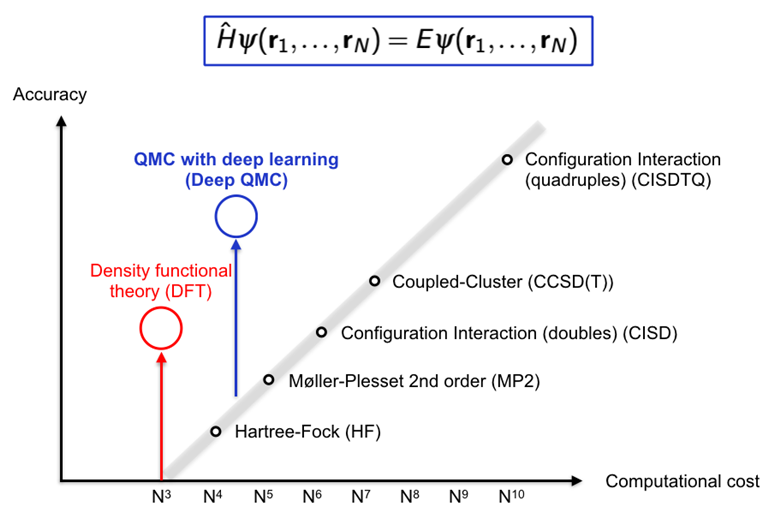
\includegraphics[width=0.8\linewidth]{fig/qm_scaling.png}
    \caption{แผนภาพแสดง Scaling ของวิธีทางเคมีควอนตัม (เครดิตภาพ: https://www.chemistryworld.com/)}
    \label{fig:qm_scaling}
\end{figure}

\begin{table}[H]
    \centering
    \caption{ตารางเปรียบเทียบความซับซ้อนเชิงคำนวณของวิธีทางเคมีควอนตัม\autocite{rupp2015} โดย $N$ คือจำนวนของอิเล็กตรอนหรือ%
    จำนวนของ Basis function}
    \label{tab:qm_complx}
    \small
    \begin{tabular}{lll}\toprule
    ตัวย่อ &วิธี &Runtime \\\midrule
    FCI &Full Configuration Interaction (CISDTQ) &$\mathcal{O}(N^{10})$ \\
    CC &Coupled Cluster (CCSDT) &$\mathcal{O}(N^{8})$ \\
    CC &Coupled Cluster (CCSD(T)) &$\mathcal{O}(N^{7})$ \\
    CC &Coupled Cluster (CCSD) &$\mathcal{O}(N^{6})$ \\
    FCI &Full Configuration Interaction (CISD) &$\mathcal{O}(N^{6})$ \\
    MP2 &M$\o$llor-Plesset second order perturbation theory &$\mathcal{O}(N^{5})$ \\
    QMC &Quantum Monte Carlo &$\mathcal{O}(N^{3}) - \mathcal{O}(N^{4})$ \\
    HF &Hartree-Fock &$\mathcal{O}(N^{3}) - \mathcal{O}(N^{4})$ \\
    DFT &Density Functional Theory (Kohn-Sham) &$\mathcal{O}(N^{3})$ \\
    TB &Tight Binding &$\mathcal{O}(N^{3})$ \\
    MM &Molecular Mechanics &$\mathcal{O}(N^{2})$ \\
    \bottomrule
    \end{tabular}
\end{table}

ตารางที่ \ref{tab:qm_complx} แสดงค่าความซับซ้อนของการคำนวณ (Compuational Complexity) ของแต่ละวิธี โดยจะเห็นได้ว่าวิธี DFT 
นั้นมีความซับซ้อนคือ $\mathcal{O}(N^{3})$ นั่นคือมันเป็นสัดส่วนโดยตรงกับจำนวนของอิเล็กตรอนของระบบ ($N$) ยกกำลังสาม ซึ่งมาจาก%
การที่เราจะต้องทำการ Diagonalize Hamiltonian ซึ่งความซับซ้อนของ Diagonalization สำหรับเมทริกซ์จตุรัสขนาด $n \times n$ คือ 
$\mathcal{O}(n^{3})$

\begin{adjustwidth}{-2.5 cm}{-2.5 cm}
    \centering
    \begin{threeparttable}[H]
    \caption{ตารางเปรียบเทียบความซับซ้อนเชิงคำนวณของวิธีทางเคมีควอนตัม\autocite{zotero-328} โดย $n$ คือจำนวนของข้อมูล $p$ 
    คือจำนวน Feature $n_{trees}$ คือจำนวนของต้นไม้ (Trees) $n_{sv}$ คือจำนวนของ Support Vectors $n_{L_{i}}$ 
    คือจำนวนของ Neuron หรือ Node ของชั้นที่ $i$ และ $t$ คือจำนวนของ Epochs ที่ใช้ในการเทรน Model}
    \label{tab:ml_complx}
    \small
    \begin{tabular}{lll}\toprule
    \multirow{2}{*}{อัลกอริทึม} &\multicolumn{2}{c}{Runtime} \\\cmidrule{2-3}
    &การเทรนโมเดล &การทำนายเอาต์พุต\\\midrule
    Decision Tree &$\mathcal{O}(n^{2}p)$ &$\mathcal{O}(p)$ \\
    Random Forest &$\mathcal{O}(n^{2}pn_{trees})$ &$\mathcal{O}(pn_{trees})$ \\
    Gradient Boosting (n\_{trees}) &$\mathcal{O}(npn_{trees})$ &$\mathcal{O}(pn_{trees})$ \\
    Linear Regression &$\mathcal{O}(p^{2}n+p^{3})$ &$\mathcal{O}(p)$ \\
    SVM (Kernel) &$\mathcal{O}(n^{2}p+n^{3})$ &$\mathcal{O}(n_{sv}p)$ \\
    Neural Network &$\mathcal{O}(npt*(n_{L_{1}}n_{L_{2}}+ n_{L_{2}}n_{L_{3}} + \dots)$ &$\mathcal{O}(pn_{L_{1}} 
    + n_{L_{1}}n_{L_{2}}+ \dots)$ \\
    \bottomrule
    \end{tabular}
\end{threeparttable}
\end{adjustwidth}

ตารางที่ \ref{tab:ml_complx} แสดงค่าความซับซ้อนของการคำนวณของอัลกอริทึม ML แบบต่าง ๆ เช่นเดียวกับตารางก่อนหน้านี้ 
โดยอัลกอริทึมที่แสดงนั้นถูกใช้กับโจทย์ปัญหา Classification และ Regression (ยกเว้น Linear Regression ที่ใช้สำหรับ Regression 
เท่านั้น) จะเห็นได้ว่าความซับซ้อนของวิธี ML นั้นจะขึ้นอยู่กับจำนวนของข้อมูลและจำนวน Feature ของข้อมูลแต่ละตัวเป็นหลัก ยกเว้นกรณีของ
โมเดลโครงข่ายประสาท (Neural Network) หรือการเรียนรู้เชิงลึก (Deep Learning) เท่านั้นที่ความซับซ้อนของมันจะขึ้นอยู่กับจำนวนรอบที่ใช้%
ในการฝึกสอน (เทรน) โมเดลและจำนวนชั้นของโครงข่าย

ถ้าหากเปรียบเทียบแล้วจะพบว่าวิธี ML นั้นมีความซับซ้อนน้อยกว่าวิธี QM อย่างมีนัยสำคัญ อย่างน้อย ๆ ก็ในระดับหลายเท่าตัว และยิ่งไปกว่านั้น
ความซับซ้อนเชิงการคำนวณในการทำนายค่าเอาต์พุตของโมเดลที่ผ่านการฝึกสอนมาแล้วนั้นต่ำมาก ซึ่งโดยส่วนใหญ่แล้วจะอยู่ในรูปของผลคูณ%
เชิงเส้นแบบดีกรี 1 ระหว่างจำนวนของข้อมูลกับจำนวนของ Feature นี่จึงเป็นเหตุผลที่ทำให้งานวิจัยทางด้านเคมี โดยเฉพาะด้าน QM ในช่วงระยะเวลา
10 ปีที่ผ่านมานั้น นักวิจัยเริ่มให้ความสนใจในการประยุกต์ใช้ ML เพื่อมาใช้ในการสร้างโมเดลสำหรับประมาณค่าหรือทำนายค่าต่าง ๆ ทางควอนตัม 
นั่นก็เพราะ ML เป็นวิธีที่สิ้นเปลืองน้อยกว่า

%--------------------------
\section{ทักษะที่จำเป็นสำหรับผู้เริ่มต้นศึกษาการเรียนรู้ของเครื่อง}
%--------------------------

การมีความรู้พื้นฐานก่อนเริ่มศึกษา ML อย่างจริงจังนั้นมันเป็นสิ่งสำคัญ ผู้เขียนได้สรุป 5 สิ่งสำคัญที่ผู้ที่เริ่มต้นศึกษาควรจะต้องรู้ ดังต่อไปนี้

\begin{enumerate}
    \item \textbf{พีชคณิตเชิงเส้นและแคลคูลัสแบบหลายตัวแปร} : ทั้งสองวิชานี้ถือว่าเป็นรากฐานของ ML เลยก็ว่าได้ 
    เพราะว่าโมเดลทุกรูปแบบของ ML นั้นต่างก็ล้วนแต่เป็นคณิตศาสตร์ ถ้าหากเราต้องการที่จะพัฒนาอัลกอริทึมใหม่ ๆ 
    หรือปรับปรุงอัลกอริทึมที่มีอยู่แล้ว เราจะต้องอาศัยความรู้พีชคณิตเชิงเส้น (เวกเตอร์และเมทริกซ์) และแคลคูลัส (การหาอนุพันธ์) 
    แต่ถ้าหากว่าเราเน้นไปทางสายแอพพลิเคชัน เราก็อาจจะไม่จำเป็นต้องรู้แบบลึกหรือละเอียดมากก็ได้ เพราะว่าในปัจจุบันมีเครื่องมือและไลบรารี่%
    สำเร็จรูปให้เราเลือกใช้มากมาย
    \item \textbf{สถิติ} : เนื่องจากว่าในขั้นตอนก่อนที่จะเริ่มสร้างและเทรนโมเดล ML นั้น เราจะต้องใช้เวลาส่วนใหญ่ 
    (อาจจะมากถึง 80\%) ไปกับการรวบรวมข้อมูล ทำความสะอาดข้อมูล การศึกษาการกระจายตัวของข้อมูล การตั้งและทดสอบสมมติฐาน 
    การทำการถดถอย (Regression) การแยกประเภท (Classification) เราจึงจำเป็นจะต้องใช้สถิติเข้ามาช่วยเพื่อให้เข้าใจถึงรายละเอียด
    ของชุดข้อมูลที่เรากำลังจะเล่นกับมัน ยิ่งเข้าใจข้อมูลมากเท่าไหร่ ยิ่งช่วยให้เราสามารถเลือกใช้โมเดล ML ได้เหมาะสมเท่านั้น 
    \item \textbf{โปรแกรมมิ่ง} : สิ่งสำคัญลำดับถัดมาคือทักษะในการเขียนโปรแกรมหรือเขียนโค้ด ถึงแม้ว่าเราจะมีความรู้ด้านทฤษฎีที่แม่นยำ 
    แต่ถ้าหากเราไม่สามารถเขียนโปรแกรมได้ แล้วก็ไม่สามารถสร้างโมเดลหรือนำ ML มาใช้งานจริงได้เลย ดังนั้นเราควรจะต้องเรียนรู้การเขียนโปรแกรม
    ให้ได้อย่างน้อยสัก 1 ภาษา ซึ่งภาษาที่ได้รับความนิยมมากที่สุดสำหรับงานทางด้านวิทยาศาสตร์ข้อมูล ณ ตอนนี้คือภาษา Python 
    นั่นก็เพราะตัวภาษาเองมี Syntax ที่ง่าย มี Library ให้เลือกใช้เยอะ มี Community ที่ใหญ่มาก ไม่ต้องกลัวเลยว่าถ้าหากมีปัญหา%
    เกี่ยวกับการเขียน Python แล้วจะไม่มีคนช่วยหรือหาวิธีแก้ปัญหาไม่ได้
    \item \textbf{แนวคิดของ ML} : แนวคิดหรือ Concept ทางด้าน ML (วิทยาศาสตร์ข้อมูล) เป็นสิ่งที่สำคัญมากเช่นเดียวกัน
    เราควรจะทราบคำศัพท์เฉพาะทางและความหมาย (Terminology) ประเภทของ ML แนวทางการนำ ML มาใช้ (Best Practice)
    \item \textbf{ฝึกทำโจทย์จริง} : ตัวช่วยที่ดีที่สุดให้เราเรียนรู้ ML ได้ง่ายและเร็วนั่นก็คือการฝึกฝน ลองหาโจทย์จริง ๆ มาฝึกทำ
    หรืออาจจะลองเก็บเกี่ยวประสบการณ์โดยเข้าร่วมการแข่งขันวิทยาศาสตร์ข้อมูล ซึ่ง ณ ปัจจุบันก็มีการจัดแข่งขันบ่อยมาก ๆ เรียกได้ว่ามีสนาม
    ให้ได้ฝึกฝนวิทยายุทธเป็นพัน ๆ เลย เช่น Kaggle\footnote{\url{https://www.kaggle.com/competitions}} และ
    AIcrowd\footnote{\url{https://www.aicrowd.com}} 
\end{enumerate}

%--------------------------
\section{แนวทางสำหรับการศึกษาการเรียนรู้ของเครื่อง}
%--------------------------

ผู้เขียนได้สรุปแนวทางศึกษา ML สำหรับงานวิจัยทางด้านเคมี (เน้นเคมีควอนตัม) สำหรับผู้เริ่มต้นตามด้านล่างต่อไปนี้
\footnote{แนวทางดังกล่าวเป็นความคิดเห็นส่วนตัวของผู้เขียนซึ่งอ้างอิงตามประสบการณ์จริง นอกจากแหล่งความรู้ที่ผู้เขียนได้แนะนำไว้แล้วจริง ๆ 
ยังมีแหล่งความรู้อื่น ๆ อีกมากมายที่ผู้อ่านสามารถศึกษาตามได้ด้วยตัวเอง}

\begin{enumerate}
    \item เริ่มจากปรับพื้นฐานพีชคณิตเชิงเส้น (โดยเน้นไปที่เมทริกซ์) และแคลคูลัสแบบหลายตัวแปร เช่น การหาอนุพันธ์ย่อย รวบไปถึงวิธีวิเคราะห์ทางสถิติ
    \item เรียนคอร์สปัญญาประดิษฐ์เบื้องต้น โดยคอร์สที่ผมแนะนำคือคอร์สออนไลน์ของ Prof. Andrew Ng บน Coursera โดยมีสองคอร์สหลักคือ 
    1. Machine Learning Specialization\footnote{\url{https://www.coursera.org/specializations/machine-learning-introduction}} และ 
    2. Deep Learning Specialization\footnote{\url{https://www.coursera.org/specializations/deep-learning}}
    \item ทำแบบฝึกหัดตามหนังสือ \enquote{Hands-on machine learning with scikit-learn, keras, and tensorflow} และ/หรือ 
    หนังสือ \enquote{Python Machine Learning} เพื่อจะได้ทำความคุ้นเคยกับ Framework ในการเขียนโค้ด ML และ DL
    \item ศึกษาการประยุกต์ ML และ DL สำหรับเคมีด้วยเว็บไซต์ \url{https://dmol.pub} ที่จัดทำโดยกลุ่มวิจัยของ Prof. Andrew White 
    ซึ่งจะมีโจทย์ทางเคมีให้ เช่น การทำนายคุณสมบัติที่สำคัญของโมเลกุล การทำนายพลังงานรวม
    \item ทบทวนงานวิจัย (Literature Review) ในวารสารวิชาการที่อ่านได้ง่าย ไม่ลงรายละเอียดเชิงเทคนิคมากไป เช่น Chemical Reviews 
    ที่เกี่ยวกับ ML in Chemistry
    \item เลือกอ่านบทความงานวิจัยจากวารสานเฉพาะทางทางด้านเคมีทฤษฎี โดยเลือกหัวข้องานวิจัยเคมีที่เราสนใจนำ ML ไปประยุกต์ใช้กับหัวข้อนั้น ๆ
\end{enumerate}

%--------------------------
\section{คำศัพท์เฉพาะทางด้านการเรียนรู้ของเครื่อง}
%--------------------------

\begin{description}[style=nextline]
    \item[Accuracy] ค่าความถูกต้องของการทำนายของโมเดล ส่วนมักมักจะรายงานค่าความถูกต้องเป็นเปอร์เซ็นต์
    \idxboth{ค่าความถูกต้อง}{Accuracy}

    \item[Algorithm] วิธีหรือขั้นตอนกระบวนการคิดคำนวณทางคณิตศาสตร์เพื่อให้ได้ผลลัพธ์ออกมา
    \idxboth{อัลกอริทึม}{Algorithm}

    \item[Attribute] ปริมาณที่ได้จากการสังเกตซึ่งบ่งบอกถึงคุณลักษณะของสิ่งที่สนใจ เช่น สี, ขนาด, ความสูง พูดง่่าย ๆ คือถ้าเป็นชุดข้อมูล 
    Attribute ก็คือชื่อของแต่ละคอลัมน์นั่นเอง
    \idxboth{คุณลักษณะ}{Attribute}

    \item[Categorical Variables] ตัวแปรจัดกลุ่ม ไม่มีความต่อเนื่อง เป็นข้อมูลประเภทแบบแยกออกจากกันและไม่ขึ้นต่อค่าอื่น ๆ เช่น 
    เพศ เชื้อชาติ พันธ์สุนัข ชนิดของผลไม้ ชนิดของหมู่ฟังก์ชันในโมเลกุล
    \idxboth{ตัวแปรจัดกลุ่ม}{Categorical Variables}

    \item[Classification] การจำแนกข้อมูลหรือการทำนายค่าที่มีความไม่ต่อเนื่อง เช่น ประเภทของยานพาหนะ ชนิดของผลไม้
    \idxboth{การจำแนก}{Classification}
 
    \item[Clustering] การจัดกลุ่มข้อมูล
    \idxboth{การจัดกลุ่ม}{Clustering}

    \item[Confusion matrix] เมทริกซ์ที่แสดงการประเมินผลลัพธ์ของการทำนาย
    \begin{itemize}
        \item True Positives (TP): ทำนายว่าจริง และสิ่งที่เกิดขึ้นก็จริง
        \item True Negatives (TN): ทำนายว่าไม่จริง และสิ่งที่เกิดขึ้นก็ไม่จริง
        \item False Positives (FP): ทำนายว่าจริง แต่สิ่งที่เกิดขึ้นคือไม่จริง
        \item False Negatives (FN): ทำนายว่าไม่จริง แต่สิ่งที่เกิดขึ้นคือจริง
    \end{itemize}
    \idxen{Confusion matrix}

    \item[Continuous Variables] ตัวแปรต่อเนื่อง เป็นตัวแปรเชิงปริมาณที่มีค่าในช่วงที่กำหนด เช่น น้ำหนัก จำนวนรถ ความยาวพันธะ
    \idxboth{ตัวแปรต่อเนื่อง}{Continuous Variables}

    \item[Convergence] สถานะของโมเดลเมื่อการเปลี่ยนของค่า Loss ระหว่าง Interation มีขนาดน้อยมาก ๆ
    \idxboth{การลู่เข้า}{Convergence}

    \item[Data Set หรือ Dataset] ชุดข้อมูลที่ได้เตรียมไว้ ประกอบไปด้วยข้อมูลอินพุต (Input) และ/หรือเอาต์พุต (Output)
    \idxboth{ชุดข้อมูล}{Data Set}

    \item[Descriptor] วิธีที่ใช้ในการแปลงข้อมูล เช่น ข้อมูลของโครงสร้างโมเลกุล ให้เป็นข้อมูลเวกเตอร์ที่เป็น Feature
    \idxen{Descriptor}

    \item[Epoch] จำนวนครั้งหรือจำนวนรอบที่อัลกอริทึมมองเห็นหรือได้รับชุดข้อมูลทั้งหมดเข้ามาเพื่อทำการเรียนรู้
    \idxen{Epoch}

    \item[Extrapolation] เป็นการทำนายที่อยู่นอกเหนือจากชุดข้อมูลที่ใช้ในการฝึกสอนโมเดล
    \idxen{Extrapolation}

    \item[Feature] คุณลักษณะเฉพาะของสิ่งที่สนใจ โดยเป็นข้อมูลแบบ 1 มิติที่ถูกสร้างโดย Descriptor
    \idxboth{คุณลักษณะเฉพาะ}{Feature}

    \item[Hyperparameter] พารามิเตอร์ขั้นสูงที่กำหนดคุณสมบัติของโมเดล เช่น ความเร็วในการเรียนรู้ ความซับซ้อนของโมเดล
    ซึ่งผู้ใช้งานจะต้องทำการกำหนดพารามิเตอร์เหล่านี้ก่อนทำการสร้างหรือฝึกสอนโมเดล
    \idxboth{ไฮเปอร์พารามิเตอร์}{Hyperparameter}

    \item[Learning Rate] อัตราเร็วในการเรียนรู้ของโมเดล หรือในทางทฤษฎีคือขนาดของก้าวในการปรับปรุง (Update Step) ในกระบวนการ 
    Optimization โดยการใช้อัลกอริทึม เช่น Gradient Descent
    \idxboth{อัตราเร็วในการเรียนรู้}{Learning rate}

    \item[Loss] ค่าความคลาดเคลื่อนหรือความแตกต่างระหว่างค่าที่ได้จากการทำนาย (Prediction) และค่าอ้างอิง (Ground Truth หรือ 
    Reference) ยิ่ง Loss มีค่าน้อย หมายความว่าโมเดลของเรายิ่งมีประสิทธิภาพสูง โดยค่า Loss จะถูกคำนวณในระหว่างการฝึกสอนโมเดล
    \idxboth{ค่่าความคลาดเคลื่อน}{Loss}

    \item[Model] ชุดคำสั่งหรือโปรแกรมที่ถูกสร้างขึ้นมาโดยมีความสามารถในการคำนวณ ประมวลผลและตัดสินใจ
    \idxboth{แบบจำลอง}{Model}

    \item[Noise] ข้อมูลที่มีความผิดปรกติและไม่มีความเกี่ยวข้องกับข้อมูลที่เราสนใจ รวมไปถึงค่าที่เกิดจากการสุ่ม (Randomness)

    \item[Normalization] การทำให้เป็นปรกติ เป็นการกำหนดหรือบังคับค่าของน้ำหนัก (Weights) ในการทำ Regression เพื่อป้องกันปัญหา
    Overfitting (การ Fit ข้อมูลที่ดีเกินไป) และเพิ่มความเร็วในการคำนวณ
    \idxboth{การทำให้เป็นปรกติ}{Normalization}

    \item[Outlier] ค่าที่ผิดปกติไปจากข้อมูลตัวอื่นในชุดข้อมูล
    \idxen{Outlier}

    \item[Overfitting] คือการที่โมเดลที่ถูกฝึกสอนด้วยชุดข้อมูล Training Set มีค่าความถูกต้องในการบ่งบอกคลาสเป้าหมายสูง 
    แต่เมื่อนำไปใช้กับข้อมูลทดสอบ Test Set กลับได้ค่าความถูกต้องต่ำ กล่าวอีกนัยหนึ่งคือตัวโมเดลที่ได้สามารถเรียนรู้ข้อมูลจาก Training Set 
    ได้ดีมาก แต่ไม่สามารถนำไปใช้กับข้อมูลใหม่ที่ไม่เคยพบมาก่อน (Unknown Data) ได้ดี
    \idxen{Overfitting}

    \item[Parameter] คุณสมบัติของข้อมูลที่ถูกเรียนรู้โดยโมเดลปัญญาประดิษฐ์ โดยพารามิเตอร์จะถูกปรับให้มีความเหมาะสมตามอัลกอริทึมที่ใช้
    เช่น Optimization ตัวอย่างของพารามิเตอร์มีดังนี้
    \begin{itemize}
        \item น้ำหนัก (Wegiths) ในเทคนิค Neural Network
        \item Support vectors ในเทคนิค Support Vector Machine
        \item ค่าสัมประสิทธิ์ (Coefficients) ในเทคนิค Linear Regression
    \end{itemize}
    \idxboth{พารามิเตอร์}{Parameter}

    \item[Precision] ความแม่นยำของการทำนาย มีสูตรในการคำนวณดังนี้
    \begin{equation}\label{eq:precision}
        P = \frac{\text{True Positives}}{\text{True Positives} + \text{False Positives}}
    \end{equation}

    \item[Prediction] กระบวนการทำนายค่าของโมเดลโดยจะทำนายค่าเอาต์พุตของข้อมูลใหม่ที่ถูกป้อนเข้าไป
    \idxboth{การทำนาย}{Prediction}

    \item[Regression]  การทำนายค่าที่มีความต่อเนื่อง เช่น ราคาสินค้า ปริมาณน้ำมัน ถ้าในบริบทของเคมีก็จะเป็นคุณสมบัติของโมเลกุล 
    เช่น พลังงานภายในของโมเลกุล, พลังงานอิสระของโมเลกุล และพลังงานกระตุ้น
    \idxen{Regression}

    \item[Regularization] การทำให้ถูกต้อง เป็นเทคนิคสำหรับการแก้ปัญหา Overfitting โดยการเพิ่มพจน์พิเศษที่มีความซับซ้อนเข้าไปใน 
    Loss function โดยเทคนิคนี้มีประโยชน์อย่างมากในการสร้างโมเดลที่มีความซับซ้อน
    \idxboth{การทำให้ถูกต้อง}{Regularization}

    \item[Reinforment Learning] การเรียนรู้แบบเสริมแรง 
    \idxboth{การเรียนรู้แบบเสริมแรง}{Reinforment Learning}

    \item[Representation] Feature ของโมเลกุลในรูปแบบสัญลักษณ์ (Symbolic) เช่น SMILES, InChI, สูตรโมเลกุล
    \idxen{Representation}

    \item[Segmentation] กระบวนการหรือขั้นตอนการแบ่งส่วนของชุดข้อมูลออกเป็นหลาย ๆ ชุดข้อมูลย่อย
    \idxen{Segmentation}

    \item[Specificity] ความจำเพาะเจาะจง เป็นพารามิเตอร์ที่วัเประสิทธิภาพของโมเดลในการจำแนกกรณีที่เป็นเท็จหรือไม่เป็นจริง (Negative)
    กล่าวอีกอย่างคือ เมื่อคำตอบคือ Negative พารามิเตอร์ตัวนี้จะบอกเราว่าการทำนายของโมเดลของเรานั้นถูกต้องมากน้อย (บ่อย) แค่ไหน
    โดยมีสูตรในการคำนวณคือ
    \begin{equation}\label{eq:specficity}
        S = \frac{\text{True Negatives}}{\text{True Negatives} + \text{False Positives}}
    \end{equation}
    \idxboth{ความจำเพาะเจาะจง}{Specificity}

    \item[Supervised Learning] การเรียนรู้ของโมเดลแบบมีผู้สอน (Output)
    \idxboth{การเรียนรู้แบบมีผู้สอน}{Supervised Learning}

    \item[Target / Output / Class / Label] คำตอบหรือเป้าหมายที่ต้องการคำนวณ ประมาณค่า หรือทำนาย
    \idxen{Target}
    \idxen{Output}
    \idxen{Class}
    \idxen{Label}

    \item[Test Set] ชุดข้อมูลที่ใช้ทดสอบความถูกต้องและแม่นยำของ Model
    \idxboth{ชุดข้อมูล!ชุดข้อมูลสำหรับการทดสอบ}{Test Set}

    \item[Training] กระบวนการสร้างและฝึกสอนโมเดลโดยใช้ Training set 
    \idxboth{การฝึกสอน}{Training}

    \item[Training Set] ชุดข้อมูลที่นำมาใช้ในการสอนคอมพิวเตอร์เพื่อสร้าง Model
    \idxboth{ชุดข้อมูล!ชุดข้อมูลสำหรับการฝึกสอน}{Training Set}

    \item[Transfer Learning] การเรียนรู้แบบส่งต่อ เป็นการนำโมเดล ML ที่ผ่านการฝึกสอนแล้วและสามารถทำงานอย่างหนึ่งได้อยู่แล้วมาฝึกสอน%
    อีกครั้งหนึ่งเพื่อให้สามารถทำงานที่สองได้ โดยวิธีการทำ Transfer Learning ก็คือเรานำค่าพารามิเตอร์ที่ถูกปรับโดยผ่านการฝึกสอนแล้ว
    เช่น น้ำหนัก นำมาใช้ต่อในการทำนายค่าอื่น ๆ นั่นเอง
    \idxboth{การเรียนรู้แบบส่งต่อ}{Transfer Learning}

    \item[Unsupervised Learning] การเรียนรู้ของโมเดลแบบไม่มีผู้สอน (Output-free)
    ซึ่งยังสามารถแบ่งออกได้เป็นสองประเภทคือ 1. Binary Classification กับ 2. Multi-class Classification
    \idxboth{การเรียนรู้แบบมีไม่มีผู้สอน}{Unsupervised Learning}

    \item[Validation Set] ชุดข้อมูลสำหรับประเมินประสิทธิภาพของโมเดลก่อนที่จะนำไปทดสอบกับ Test Set จริง 
    โดย Data Set ประเภทนี้มักจะถูกนำมาใช้ในการทำ Cross-validation
    \idxboth{ชุดข้อมูล!ชุดข้อมูลสำหรับการประเมินผล}{Validation Set}
\end{description}
